\documentclass[12pt]{article}
\usepackage{graphicx}
\usepackage{../lp}
% Cross-references for handout numbers.
\usepackage{amsfonts}
%\usepackage{amsthm}
\usepackage{hyperref}
\usepackage{amssymb}
%\usepackage[capitalize]{cleveref}
\usepackage{xcolor}

%\input{handouts}

\newcounter{chapnum}

\newtheorem{definition}{Definition}[chapnum]
\newtheorem{remark}{Remark}[chapnum]
\newtheorem{theorem}{Theorem}[chapnum]
\newtheorem{lemma}[theorem]{Lemma}
\newtheorem{corollary}[theorem]{Corollary}
\newtheorem{proposition}[theorem]{Proposition}
\newtheorem{claim}[theorem]{Claim}
\newtheorem{observation}{Observation}[chapnum]

\renewcommand{\thesection}{\arabic{chapnum}.\arabic{section}}
\renewcommand{\thefigure}{\arabic{chapnum}.\arabic{figure}}


\newenvironment{proof}{\noindent{\bf Proof:} \hspace*{1em}}{
        \hspace*{\fill} $\triangle$ }
\newenvironment{proof_of}[1]{\noindent {\bf Proof of #1:}
        \hspace*{1em} }{\hspace*{\fill} $\triangle$ }
\newenvironment{proof_claim}{\begin{quotation} \noindent}{
        \hspace*{\fill} $\diamond$ \end{quotation}}
\newenvironment{solution}{\noindent{\bf Solution:} \hspace*{1em}}{
        \hspace*{\fill} $\triangle$ }


\newcommand{\R}{{\mathbb R}}
\newcommand{\Z}{{\mathbb Z}}
\newcommand{\Q}{{\mathbb Q}}
\newcommand{\C}{{\mathbb C}}
\newcommand{\N}{{\mathbb N}}
\newcommand{\lin}{\operatorname{lin}}
\newcommand{\aff}{\operatorname{aff}}
\newcommand{\cone}{\operatorname{cone}}
\newcommand{\conv}{\operatorname{conv}}
\newcommand{\vol}{\operatorname{vol}}
\newcommand{\poly}{\operatorname{poly}}




\newcommand{\CF}[1]{{\color{purple}[CF: #1]}}


\newlength{\toppush}
\setlength{\toppush}{2\headheight}
\addtolength{\toppush}{\headsep}

\newcommand{\htitle}[2]{\noindent\vspace*{-\toppush}\newline\parbox{6.5in}
{Massachusetts Institute of Technology \hfill 18.453: Combinatorial Optimization 
\newline
\textbf{Instructor:} Cole Franks \quad \textbf{Notes: }Michel Goemans and Zeb Brady \hfill#2\newline
\mbox{}\hrulefill\mbox{}}\vspace*{1ex}\mbox{}\newline
\begin{center}{\Large\bf #1}\end{center}}

\newcommand{\handout}[2]{\thispagestyle{empty}
 \markboth{ #1 \hfil #2}{ #1 \hfil #2}
 \pagestyle{myheadings}\htitle{#1}{#2}}


\setlength{\oddsidemargin}{0pt}
\setlength{\evensidemargin}{0pt}
\setlength{\textwidth}{6.5in}
\setlength{\topmargin}{0in}
\setlength{\textheight}{8.5in}


\newcounter{exercisenum}
\newcounter{exercisetot}
\setcounter{exercisetot}{0}



\newenvironment{exercises}{
	\begin{list}{{\bf Exercise \arabic{chapnum}-\arabic{exercisenum}. \hspace*{0.5em}}}
	{\setlength{\leftmargin}{0em}
	 \setlength{\rightmargin}{0em}
	 \setlength{\labelwidth}{0em}
	 \setlength{\labelsep}{0em}
	\usecounter{exercisenum}
      \setcounter{exercisenum}{\theexercisetot}}}{\setcounter{exercisetot}{\theexercisenum}\end{list}}


\newenvironment{pseudocode}{
    \begin{list}{}{
        \renewcommand{\makelabel}{$\triangleright$}
        \setlength{\topsep}{0pt}
        \setlength{\leftmargin}{32pt}
        \setlength{\labelwidth}{14pt}
        \setlength{\labelsep}{0mm}
        \setlength{\itemindent}{0mm}
        \setlength{\itemsep}{-3pt}
        \setlength{\itemsep}{0mm}
        \setlength{\parsep}{0pt}%
        \setlength{\listparindent}{0pt}
    }
}
{
    \end{list}
}

\usepackage{amsmath}

\setcounter{chapnum}{7}


\begin{document}


\handout{\arabic{chapnum}. Lecture notes on the ellipsoid algorithm}{} 

The simplex algorithm was the first algorithm proposed for linear
programming, and although the algorithm is quite fast in practice, no
variant of it is known to be polynomial time. The Ellipsoid algorithm
is the first polynomial-time algorithm discovered for linear
programming. The Ellipsoid algorithm was proposed by the Russian mathematician
Shor in 1977 for general convex optimization problems, and applied to
linear programming  by Khachyan in 1979. Contrary to the simplex
algorithm, the ellipsoid algorithm is not very fast in practice;
however, its theoretical polynomiality has important consequences for
combinatorial optimization problems as we will see. Another
polynomial-time algorithm, or family of algorithms to be more precise,
for linear programming is the class of interior-point algorithms that
started with Karmarkar's algorithm in 1984; interior-point algorithms
are also quite practical but they do not have the same important
implications to combinatorial optimization as the ellipsoid algorithm
does. 

The problem being considered by the ellipsoid algorithm is:
\begin{quote}
Given a bounded convex set $P\in \R^{n}$ find $x \in P$. 
\end{quote}

We will see that we can reduce linear programming  to finding an $x$
	in $P=\{x\in \R^{n} : Cx \leq d\}$.

The ellipsoid algorithm works as follows. We start with a big
ellipsoid $E$ that is guaranteed to contain $P$. We then check if the
center of the ellipsoid is in $P$. If it is, we are done, we found a
point in $P$. Otherwise, we find an inequality $c^Tx \leq d_i$ which
is satisfied by all points in $P$ (for example, it is explicitly given
in the description of $P$) which is not satisfied by our center. $P$ is then contained in the body $E \cap \{x: c^Tx \leq d_i\}$, which is some piece of the ellipsoid $E$. We find a new ellipsoid $E'$ containing $E \cap \{x: c^Tx \leq d_i\}$, replace $E \leftarrow E'$ and repeat the process. Critically, we will always be able to find $E'$ with volume a constant (but dimension-dependent) factor smaller than that of $E$. Because the volume of $E$ can never be smaller than that of $K$, the number of steps before the center is in $P$ is at most $\poly(n)\log \frac{\vol(E)}{\vol(P)}.$
One iteration of the ellipsoid algorithm is illustrated in Figure
\ref{ellip}. The ellipsoid algorithm is the following. 

\begin{itemize}
\item
	Let $E_0$ be an ellipsoid containing P
\item
	while center $a_k$ of $E_k$ is not in $P$ do:
\begin{itemize}
\item
Let $c^{T}x \leq c^{T}a_k$ be such that $\{x:c^Tx\leq c^Ta_k\}\supseteq P$
\item
Let $E_{k+1}$ be the minimum volume ellipsoid containing $E_k \cap
\{x:c^Tx\leq c^{T}a_k\}$
\item
$k \leftarrow k+1$
\end{itemize}
\end{itemize}

\begin{figure}[htbp]
\begin{center}
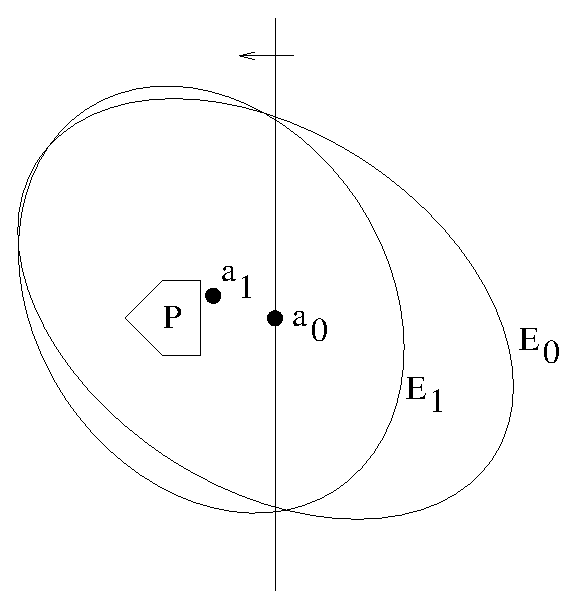
\includegraphics[scale=0.7]{../figures/ellipsoid}
\end{center}
\caption{One iteration of the ellipsoid algorithm. }
\label{ellip}
\end{figure}

The ellipsoid algorithm has the important property that the ellipsoids
contructed shrink in volume as the algorithm proceeds; this is stated
precisely in the next lemma. This means that if the set $P$ has
positive volume, we will eventually find a point in $P$. We will need
to deal with the case when $P$ has no volume (i.e. $P$ has just a
single point), and also discuss when we can stop and be guaranteed
that either we have a point in $P$ or we know that $P$ is empty.  
\begin{lemma} \label{volume}
$\frac{Vol(E_{k+1})}{Vol(E_k)} < e^{-\frac{1}{2(n+1)}}$.
\end{lemma}

Before we can state the algorithm more precisely, we need to define
ellipsoids. 

\begin{definition}
Given a center $a$, and a positive definite matrix $A$, the ellipsoid 
$E(a,A)$ is defined as $\{x \in \R^n:(x-a)^T A^{-1}(x-a)\leq 1\}$. 
\end{definition}

One important fact about a positive definite matrix $A$ is that there
exists $B$ such that $A=B^TB$, and hence
$A^{-1}=B^{-1}(B^{-1})^T$. Ellipsoids are in fact just affine
transformations of unit spheres. To see this, consider the (bijective)
affine transformation $T: x \rightarrow y =(B^{-1})^T(x-a)$. It maps
$E(a,A)\rightarrow \{y:y^{T}y\leq 1\}=E(0,I)$.

We first consider the simple case in which the ellipsoid $E_k$ is the
unit sphere and the inequality we generate is $x_1\geq 0$. We
claim that the ellipsoid containing $E_k \cap \{ x:x_1\geq 0\}$ is 
$$E_{k+1}= \left\{x:
\left(\frac{n+1}{n}\right)^2\left(x_1-\frac{1}{n+1}\right)^2
+\frac{n^2-1}{n^2}\sum_{i=2}^n x_i^2 \leq 1\right\}. $$
Indeed, if we consider an $x\in E_k \cap \{x: x_1\geq 0\}$, we see
that 
\begin{eqnarray*}
\lefteqn{\left(\frac{n+1}{n}\right)^2\left(x_1-\frac{1}{n+1}\right)^2
+\frac{n^2-1}{n^2}\sum_{i=2}^n x_i^2} \\
& = & \frac{n^2+2n+1}{n^2}x_1^2
-\left(\frac{n+1}{n}\right)^2\frac{2x_1}{n+1}+\frac{1}{n^2}+ 
\frac{n^2-1}{n^2}\sum_{i=2}^n x_i^2  \\
& = &\frac{2n+2}{n^2}x_1^2 -\frac{2n+2}{n^2}x_1 +\frac{1}{n^2} +
\frac{n^2 -1}{n^2}\sum_{i=1}^n x_i^2  \\
& = & \frac{2n+2}{n^2} x_1 (x_1-1) +\frac{1}{n^2} +
\frac{n^2 -1}{n^2}\sum_{i=1}^n x_i^2  \\
&\leq& \frac{1}{n^2} + \frac{n^2 - 1}{n^2}\leq 1.
\end{eqnarray*}

In this specific case, we can prove easily lemma \ref{volume}.

\begin{proof}
The volume of an ellipsoid is proportional to the product of its side
lengths. Hence the ratio between the unit ellipsoid $E_k$ and
$E_{k+1}$ is 
\begin{eqnarray*}
\frac{Vol(E_{k+1})}{Vol{E_k}}&=&\frac{(\frac{n}{n+1}) 
(\frac{n^2}{n^2-1})^{\frac{n-1}{2}}}{1}\\
&=& \left(\frac{n}{n+1}\right)\left(\frac{n^2}{n^2-1}\right)^{\frac{n-1}{2}} \\
& < & e^{-\frac{1}{n+1}}e^{\frac{n-1}{2(n^2-1)}} = e^{-\frac{1}{n+1}}
e^{\frac{1}{2(n+1)}} = e^{-\frac{1}{2(n+1)}},
\end{eqnarray*}
where we have used the fact that $1+x \leq e^x$ for all $x$, with
strict inequality if $x\neq 0$. 
\end{proof}

Now consider the slightly more general case in which the ellipsoid is
also the unit sphere but we have an arbitrary constraint $d^Tx\leq
0$. We want to find an ellipsoid that contains $E(0, I) \cap \{x :
d^Tx \leq 0\}$ (we let $\|d\| = 1$; this can be done by scaling both
sides), it is easy to verify that we can take
$E_{k+1}=E(-\frac{1}{n+1}d, F)$, where $F = \frac{n^2}{n^2 -
1}(I-\frac{2}{n+1}d d^T)$, and the ratio of the volumes is $\leq
\exp\left(-\frac{1}{2(n+1)}\right)$.

Now we deal with the case where $E_k$ is not the unit sphere. We take
advantage of the fact that linear transformations preserve ratios of
volumes.
%
\begin{equation}
\begin{array}{ccc}
E_k & \stackrel{T}{\rightarrow} & E(0, 1)\\
 & & \downarrow \\
E_{k+1} & \stackrel{T^{-1}}{\leftarrow} & E' \\
\end{array}
\end{equation}
%
Let $a_k$ be the center of $E_k$, and $c^Tx \leq c^Ta_k$ be the
halfspace through $a_k$ that contains $P$. Therefore, the
half-ellipsoid that we are trying to contain is $E(a_k, A)\cap \{x :
c^Tx \leq c^Ta_k\}$. Let's see what happens to this half-ellipsoid
after the transformation $T$ defined by $y= T(x)=(B^{-1})^T (x-a)$. This
transformation transforms $E_k=E(a_k, A)$ to $E(0,I)$. Also,
%
\begin{equation}
\{x: c^Tx \leq c^Ta_k\}  \stackrel{T}{\rightarrow} 
\{ y: c^T(a_k +
B^Ty) \leq c^T a_k\}  = \{y: c^TB^Ty \leq 0 \} = \{y: d^Ty \leq 0\},
\end{equation}
%
where $d$ is given by the following equation:
%
\begin{equation}
d = \frac{Bc}{\sqrt{c^T B^T B c}} = \frac{Bc}{\sqrt{c^T A c}}.
\end{equation}
%
Let $b = B^Td = \frac{Ac}{\sqrt{c^T A c}}$. This implies:
%
\begin{eqnarray}
E_{k+1} & = & E\left(a_k - \frac{1}{n + 1}b, \frac{n^2}{n^2 - 1}
B^T\left(I-\frac{2}{n+1}d d^T\right)B\right) \\ 
& = & E\left(a_k - \frac{1}{n + 1}b, \frac{n^2}{n^2 -
1}\left(A-\frac{2}{n+1}bb^T\right)\right).
\end{eqnarray}
%
To summarize, here is the Ellipsoid Algorithm:
%
\begin{enumerate}
\item 
Start with $k=0$, $E_0 = E(a_0, A_0) \supseteq P$, $P = \{x : Cx \leq
d\}$.
\item While $a_k \not\in P$ do:
\begin{itemize}
\item 
Let $c^Tx \leq d$ be an inequality that is valid for all $x
\in P$ but $c^Ta_k>d$.
\item Let $b = \frac{A_kc}{\sqrt{c^TA_k c}}$.
\item Let $a_{k + 1} = a_k - \frac{1}{n+1}b$.
\item Let $A_{k + 1} = \frac{n^2}{n^2 - 1}(A_k - \frac{2}{n+1} b b^T)$.
\end{itemize}
\end{enumerate}

\begin{claim}
$\frac{Vol(E_{k+1})}{Vol(E_k)} <  \exp\left(-\frac{1}{2(n+1)}\right)$.
\end{claim}

After $k$ iterations, $Vol(E_k) \leq Vol(E_0)
\exp\left(-\frac{k}{2(n+1)}\right)$.  If $P$ is nonempty then the
Ellipsoid Algorithm should find $x \in P$ in at most $2(n+1) \ln
\frac{Vol(E_0)}{Vol(P)}$ steps. 

In general, for a full-dimensional polyhedron described as $P=\{x:
Cx\leq d\}$, one can show that $\frac{Vol(E_0)}{Vol(P)}$ is polynomial
in the encoding length for $C$ and $d$. We will not show this in
general, but we will focus on the most important situation in
combinatorial optimization when we are given a set $S\subseteq
\{0,1\}^n$ (not explicitly, but for example as the incidence vectors
of all matchings in a graph) and we would like to optimize over
$P=conv(S)$. We will make the assumption that $P$ is full-dimensional;
otherwise, one can eliminate one or several variables and obtain a
smaller full-dimensional problem. 

\paragraph{From feasibility to Optimization} 
First, let us show how to reduce such an optimization problem to the
problem of finding a feasible point in a polytope. Let $c^Tx$ with
$c\in \R^n$ be our objective function we would like to minimize over
$P$. Assume without loss of generality that $c\in \Z^n$. Instead of
optimizing, we can check the non-emptiness of 
$$P'=P\cap \{x: c^Tx\leq d+\frac{1}{2}\}$$ for $d\in \Z$ and our optimum
value corresponds to the smallest such $d$. As $S\subseteq \{0,1\}^n$,
$d$ must range in $[-n c_{max},nc_{max}]$ where $c_{max}=\max_i c_i$.
To find $d$, we can use binary search (and check the non-emptiness of
$P'$ with the ellipsoid algorithm). This will take $O(\log
(nc_{max}))=O(\log n+\log c_{max})$ steps, which is polynomial. 

\paragraph{Starting Ellipsoid.} 
Now, we need to consider using the ellipsoid to find a feasible point
in $P'$ or decide that $P'$ is empty. As starting ellipsoid, we can
use the ball centered at the vector $(\frac{1}{2}, \frac{1}{2},
\cdots, \frac{1}{2})$ and of radius $\frac{1}{2} \sqrt{n}$ (which goes
through all $\{0,1\}^n$ vectors). This ball has volume
$Vol(E_0)=\frac{1}{2^n} (\sqrt{n})^n Vol(B_n)$, where $B_n$ is the
unit ball. We have that
$Vol(B_n)=\frac{\pi^{n/2}}{\Gamma(\frac{n}{2}+1)}$, which for the
purpose here we can even use the (very weak) upper bound of
$\pi^{n/2}$ (or even $2^n$). This shows that $\log(Vol(E_0))=O(n \log n)$.

\paragraph{Termination Criterion.}
We will now argue that if $P'$ is non-empty, its volume is not too
small. Assume that $P'$ is non-empty, say $v_0\in
P'\cap\{0,1\}^n$. Our assumption that $P$ is full-dimensional implies
that there exists $v_1, v_2, \cdots, v_n\in P\cap \{0,1\}^n=S$ such
that the ``simplex'' $v_0, v_1, \cdots, v_n$ is full-dimensional. The
$v_i$'s may not be in $P'$. Instead, define $w_i$ for $i=1,\cdots,n$
by:
$$w_i =\left\{\begin{array}{ll} v_i & \mbox{if } c^Tv_i \leq
d+\frac{1}{2} \\ v_0 + \alpha (v_i-v_0) & \mbox{otherwise} \end{array}\right.$$
where $\alpha=\frac{1}{2n c_{max}}$. This implies that $w_i\in P'$ as
$$c^Tw_i = c^Tv_0 + \alpha c^T(v_i-v_0) \leq d + \frac{1}{2n c_{max}}
n c_{max} = d+\frac{1}{2}.$$ We have that $P'$ contains $C=conv(\{v_0,
w_1, w_2, \cdots, w_n\})$ and $Vol(C)$ is $\frac{1}{n!}$ times the
volume of the parallelipiped spanned by $w_i-v_0=\beta_i (v_i-v_0)$
(with $\beta_i\in \{\alpha,1\}$) for $i=1,\cdots,n$. This paralleliped
has volume equal to the product of the $\beta_i$ (which is at least
$\alpha^n$) times the volume of a parallelipiped with integer
vertices, which is at least 1. Thus,
$$Vol(P')\geq Vol(C)=\frac{1}{n!}\left(\frac{1}{2n
  c_{max}}\right)^n.$$ Taking logs, we see that the number of
  iterations of the ellipsoid algorithm before either discovering that
  $P'$ is empty or a feasible point is at most
  $$\log(Vol(E_0))-\log(Vol(P'))=O(n\log n + n \log c_{max}).$$
This is polynomial. 

\paragraph{Separation Oracle.} To run the ellipsoid algorithm, we need
to be able to decide, given $x\in \R^n$, whether $x\in P'$ or find a
violated inequality. The beauty here is that we do not necessarily
need a complete and explicit description of $P$ in terms of linear
inequalities. We will see examples in which we can even apply this to
exponential-sized descriptions. What we need is a {\it separation
  oracle} for $P$: Given $x^*\in \R^n$, either decide that $x^*\in P$ or
find an inequality $a^Tx\leq b$ valid for $P$ such that $a^Tx^*>b$. If
this separation oracle runs in polynomial-time, we have succeeded in
finding the optimum value $d$ when optimizing $c^Tx$ over $P$ (or
$S$). 

\paragraph{Finding an optimum solution.} 
There is one more issue. This algorithm gives us a point $x^*$ in $P$ of
value at most $d+\frac{1}{2}$ where $d$ is the optimum value. However,
we are interested in finding a point $x\in P\cap\{0,1\}^n=S$ of value
  exactly $d$. This can be done by starting from $x^*$ and finding
  {\it any extreme} point $x$ of $P$ such that $c^Tx\leq c^T
  x^*$. Details are omitted. 

In summary, we obtain the following important theorem shown by
Gr\"otschel, Lov\'asz and Schrijver, 1979. 

\begin{theorem}
Let $S=\{0,1\}^n$ and $P=conv(S)$. Assume that $P$ is full-dimensional
and we are given a separation oracle for $P$. Then, given $c\in \Z^n$,
one can find $\min\{c^Tx: x\in S\}$ by the ellipsoid algorithm by
using a polynomial number of operations and calls to the separation
oracle. 
\end{theorem}

To be more precise, the number of iterations of the ellipsoid
algorithm for the above application is $O(n^2 \log^2 n + n^2 \log^2
c_{max})$, each iteration requiring a call to the separation oracle
and a polynomial number of operations (rank-1 updates of the matrix
$A$, etc.).

Here are two brief descriptions of combinatorial optimization problems
that can be solved with this approach. 

\paragraph{Minimum Cost Arborescence Problem.} 

We have seen a combinatorial algorithm to solve the minimum cost
arborescence problem, and it relied on solving by a primal-dual method
the linear program: 
%
\lps & LP & = & \min & \sum_{a\in A} c_a x_a \\ \\
& \lefteqn{\mbox{subject to:}} \\ 
(P) & & & & \sum_{a\in \delta^-(S)} x_a \geq 1 & \forall S\subseteq
V\setminus\{r\} \\ 
& & & & x_a \geq 0 & a\in A.  
\elps 
%
Instead, we could use the ellipsoid algorithm to directly solve this
linear program in polynomial-time. Indeed, even though this linear
program has an exponential number of constraints (in the size of the
graph), a separation oracle for it can be easily defined. Indeed
consider $x^*$. If $x^*_a<0$ for some $a\in A$, just return the
inequality $x_a\geq 0$. Otherwise, for every $t\in V\setminus \{r\}$,
consider the minimum $r-t$ cut problem in which the capacity on arc
$a$ is given by $x^*_a$. As we have seen, this can be solved by
maximum flow computations. If for some $t\in V\setminus\{r\}$, the
minimum $r-t$ cut has value less than 1 then we have found a violated
inequality by $x^*$. Otherwise, we have that $x^*\in P$. Our
separation oracle can thus be implemented by doing $|V|-1$ maximum
flow computations, and hence is polynomial.  We are done.

\paragraph{Maximum Weight Matching Problem.} 
For the maximum weight matching problem in a general graph $G=(V,E)$,
Edmonds has shown that the convex hull of all matchings is given by:
\begin{equation}
\begin{aligned}
\sum_{e\in E(S)} x_e \leq \frac{|S|-1}{2} & \hspace*{0.5in} &  S\subset V, |S| \mbox{
  odd} \\
\sum_{e\in \delta(v)} x_e \leq 1 & \hspace*{0.5in} & v\in V \\
x_e \geq 0 & \hspace*{0.5in} & e\in E.
\end{aligned}
\end{equation}
Given $x^*$, we can easily check if $x^*$ is nonnegative and if the
$n$ constraints $\sum_{e\in \delta(v)} x_e \leq 1$ are satisfied.
There is an exponential number of remaining constraints, but we will
show now that they can be checked by doing a sequence of minimum cut
computations.

Assume $x\geq 0$ satisfies $\sum_{e\in \delta(v)} x_e \leq 1$ for
every $v\in V$, and we would like to decide if $$\sum_{e\in E(S)} x_e
\leq \frac{|S|-1}{2}$$ for all $S\subset V$, $|S|$ odd, and if not
produce such a violated set $S$. We can assume without loss of
generality that $|V|$ is even (otherwise, simply add a vertex). 
Let $$s_v=1-\sum_{e\in \delta(v)}
x_e,$$ for all $v\in V$. Observe that $\sum_{e\in E(S)} x_e
\leq \frac{|S|-1}{2}$ is equivalent to $$\sum_{v\in S} s_v +
\sum_{e\in \delta(S)} x_e \geq 1.$$ Define a new graph $H$, whose
vertex set is $V\cup \{u\}$ (where $u$ is a new vertex) and whose edge
set is $E\cup \{(u,v):v\in V\}$. In this new graph, let the capacity
$u_e$ of an edge be $x_e$ if $e\in E$ or $s_v$ for $e=(u,v)$. Observe
that in this graph, $$\sum_{v\in S} s_v +
\sum_{e\in \delta(S)} x_e \geq 1$$ if and only if $$\sum_{e\in
  \delta_H(S)} u_e \geq 1,$$ where $\delta_H(S)$ are the edges of $H$
with one endpoint in $S$. Thus, to solve our separation problem, it is
enough to be able to find the minimum cut in $H$ among all the cuts
defined by sets $S$ with $S\subseteq V$, $|S|$ odd. This is a special
case of the minimum $T$-odd cut problem seen previously. If
the minimum $T$-odd cut problem returns a minimum cut of value greater
or equal to 1, we know that all inequalities are satisfied; otherwise,
a minimum $T$-odd cut provides a violated inequality. 




\end{document}
